\section{CPU, Scheduling, and OS Services}
\label{sec:cpu}
In this section, we will measure the overhead of procedure call, system call, and the time of task creation and context switching.

\subsection{Procedure Call}
\paragraph{Methodology.} First we need to define the overhead of procedure call. We assert that the overhead of function calls stems from three key factors: 1. Preparation of function parameters; 2. The setup of the function's stack frame during the function call; 3. Function return. Considering the code in \ref{lst1}. 
\lstinputlisting[language=C++,label=lst1,caption={Non inline procedure call}]{sourcecode/CPU-Schedule-OS/latex_input/latex_lst1.c}
In System V AMD64 ABI, when calling function, the caller needs to setup the arguments for the callee, then pushes the return address and stack base pointer to the stack and jumps to the callee. When callee returns to the caller it will recover the previous stack frame and pop the return address to the program counter register to back to the caller's code. Thus, we can define the overhead of a procedure call as the additional cost incurred by three components: parameter preparation, stack frame adjustment before the jump, and stack frame adjustment upon return. To measure this overhead, we can calculate the time it takes from invoking a simplest function to its return.
\lstinputlisting[label=lst2,caption={Simplest function takes only one argument}]{sourcecode/CPU-Schedule-OS/latex_input/latex_simplest_func.asm}
By using the simplest function in \ref{lst2}, we can eliminate the performance impact brought about by compiler optimizations (e.g. inlining) and security features (e.g. stack canaries).

Before measuring procedure calls, we also need to figure out the calling conventions. In System V AMD64 ABI, Programs typically pass parameters as table \ref{table:calling-convention-reg}\footnote{We are using cdecl calling convention.}.
\begin{table}[h]
	\centering
	\begin{tabular}{c|c}
		\hline
		\bf{Arguments} & \bf{How they are passed} \\ \hline
		
		First 6 Integers & RDI, RSI, RDX, RCX, R8, R9 \\ \hline

		First 8 Floating Points & XMM0-XMM7 \\ \hline
		
		Others & Stack \\ \hline
	\end{tabular}
	\caption{\textbf{Arguments Passing in System V AMD64 Calling Convention.}}
	\label{table:calling-convention-reg}
\end{table}
From this, we can make an early prediction that, for procedure calls with integer parameters, there won't be a significant difference in calling overhead when the number of parameters is less than or equal 6. It's only when there are more than 6 parameters that significant differences may arise due to memory writes.

To measure the overhead more precisely, we use \texttt{rdtscp}\footnote{In order to preserve the execution order, we use \texttt{rdtscp} instead of \texttt{rdtsc}} instruction to read from the processor’s time-stamp counter in order to get the number of CPU cycles. In order to mitigate the impact of process scheduling, we call the same function consecutively multiple times. Also, we use \texttt{setpriority()} to raise the scheduling priority of our testing program. Before conducting the tests, we ensure that the size of the test program is smaller than a page and disable swap. This is done to maximize the likelihood of the program being fully loaded into memory during the testing process. Every testing procedure call will be executed $16777216$ times. Note that we will also measure the overhead of \texttt{rdtscp} and subtract it from the final result. 

\paragraph{Experimental results.} The result is listed in table \ref{table:procedure-test}
\begin{table}[h]
	\centering
	\begin{tabular}{c|c}
		\hline
		\bf{Arguments} & \bf{Average Cycles} \\ \hline
		0 & 5.357 (1.9 ns) \\ \hline
		1 & 5.711 (2.0 ns) \\ \hline
		2 & 7.198 (2.4 ns) \\ \hline
        3 & 4.815 (1.7 ns) \\ \hline
        4 & 6.743 (2.3 ns) \\ \hline
        5 & 5.920 (2.0 ns) \\ \hline
        6 & 4.432 (1.5 ns) \\ \hline
        7 & \textbf{11.881 (4.1 ns)} \\ \hline
        estimate of 0-6 & 5 to 10 cycles \\ \hline
        baseline of calling & 5 cycles\tablefootnote{On CPU with pipeline and superscalar\cite{superscalar}, the average cycles of a single instruction can be less than 1.} \\ \hline
	\end{tabular}
	\caption{\textbf{Average Cycles of Procedure Call.}}
	\label{table:procedure-test}
\end{table}
We have removed the overhead of \texttt{rdtscp}, which is $39.900$ cycles. 

\paragraph{Results analysis.} The result align closely with our previous predictions: when the number of parameters is between 0 and 6, there is no significant difference in overhead. Because the first 6 arguments will be passed with registers which are very efficient and much faster than memory access. It is only when memory access is required that a noticeable increase in overhead becomes apparent.

\subsection{System Call}
\paragraph{Methodology.} The overhead of a syscall, as compared to a regular procedure call, primarily arises from the context switching. Therefore, our primary task is to ascertain when will syscalls, or more frequently encountered libc syscall wrappers for usermode programmers, genuinely trap into kernel mode. We choose a simple system, clock\_gettime() to measure the overhead, by simply measuring cycles it takes to finish the system call. 

\paragraph{Virtual Syscall.} Before conducting the experiment, we need to analyze how modern Linux kernel optimize the syscall. Virtual Dynamic Shared Object, vDSO is a kernel mechanism for exporting a selected part of kernel space routines to user space. VDSO provides user mode programs with vsyscalls. These virtual syscalls eliminate the need for user mode programs to spend time on context switching for certain simple syscalls. They are the syscalls without really trapping into kernel.

\begin{lstlisting}[caption=vDSO mapping]
gef> vmmap
...
0xffffffffff600000 
0xffffffffff601000 
0x0000000000000000 --x [vsyscall]
\end{lstlisting}

\paragraph{Experimental results.} The results are in table \ref{table:syscall-test}.
\begin{table}[h]
	\centering
	\begin{tabular}{c|c|c}
		\hline
		\makecell{Type} & estimated & measured\\ \hline
        \textbf{syscall} & 1 $\mu$s & \makecell{550 ns \\ (1596.250 cycles)}  \\ \hline
        \textbf{vDSO call} & 1 $\mu$s & \makecell{24.379 ns \\ (70.699 cycles)}  \\ \hline
	\end{tabular}
	\caption{\textbf{Result of Overhead of System Call.}}
	\label{table:syscall-test}
\end{table}
We have already subtracted \texttt{rdtscp} overhead from the results. Since we have the vDSO mapping, subtracting the number of cycles required for a syscall from those needed for vDSO can provide an estimate of the overhead associated with context switching between userland and kernel mode. Thus the overhead of syscall can be calculated as follows:
\begin{equation}
    t_{\text{user\ kernel\ switch}}=t_{\text{syscall}}-t_{\text{vDSO}}=1525.550\ \text{Cycles} (526.051 ns)
\end{equation}

\paragraph{Result analysis.} As we mentioned previously, the overhead of syscall mainly consists of the context switching between userland and kernel mode. As we can tell from the table \ref{table:syscall-test}, the average cycles of vDSO call is very closed to normal procedure calling which is aligned with our predictions. By comparing vsyscall with syscall we can derive the overhead of context switching in privilege level switching.

\subsection{Task Creation} 
\paragraph{Methodology.} There are two main approaches to create a new task: \texttt{fork()} and \texttt{pthread\_create()}. Before we measure the task creation time, we should dive deeper into how these two APIs work\footnote{We are using GNU LIBC 2.38.}.

\paragraph{fork() vs. pthread\_create().} Before actually launching a task, both of these functions perform a substantial amount of preparatory work. For now, let's set aside these preparations and focus on how they each initiate a new task. Figure \ref{fig:fork-callstack} shows the call stack when calling \texttt{fork()}
\begin{figure}[htbp]
    \centering
    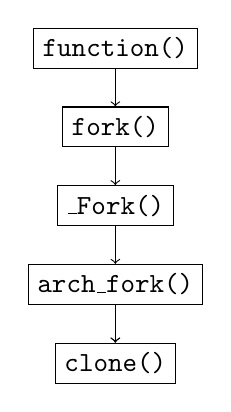
\begin{tikzpicture}[node distance=15pt]
        \node[draw] at(0, 7) (l0) {\texttt{function()}};
        \node[draw] at(0, 6) (l1) {\texttt{fork()}};
        \node[draw] at(0, 5) (l2) {\texttt{\_Fork()}};
        \node[draw] at(0, 4) (l3) {\texttt{arch\_fork()}};
        \node[draw] at(0, 3) (l4) {\texttt{clone()}};
        \draw[->] (l0)  -- (l1);
        \draw[->] (l1)  -- (l2);
        \draw[->] (l2)  -- (l3);
        \draw[->] (l3)  -- (l4);
        \draw[->] (l3)  -- (l4);
    \end{tikzpicture}
    \caption{Call Stack of \texttt{fork()}}
    \label{fig:fork-callstack}
\end{figure}
Figure \ref{fig:pthread-callstack} show the call stack when a program call \texttt{pthread\_create()} on a system that supports \texttt{clone3} syscall\footnote{Firgure 1 shows the function names instead of the versioned symbols.}.
% \lstinputlisting{assets/code/bt.c}
\begin{figure}[htbp]
    \centering
    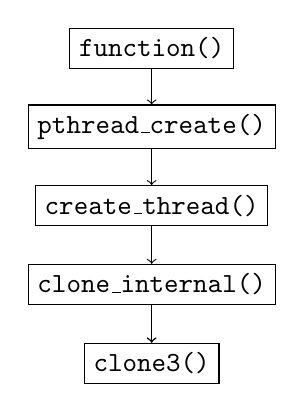
\begin{tikzpicture}[node distance=15pt]
        \node[draw] at(0, 7) (l0) {\texttt{function()}};
        \node[draw] at(0, 6) (l1) {\texttt{pthread\_create()}};
        \node[draw] at(0, 5) (l2) {\texttt{create\_thread()}};
        \node[draw] at(0, 4) (l3) {\texttt{clone\_internal()}};
        \node[draw] at(0, 3) (l4) {\texttt{clone3()}};
        \draw[->] (l0)  -- (l1);
        \draw[->] (l1)  -- (l2);
        \draw[->] (l2)  -- (l3);
        \draw[->] (l3)  -- (l4);
        \draw[->] (l3)  -- (l4);
    \end{tikzpicture}
    \caption{Call Stack of \texttt{pthread\_create()}}
    \label{fig:pthread-callstack}
\end{figure}
After calling \texttt{clone()} and \texttt{clone3()} a new task is created.
We should focus on the these two syscalls which do the job of creating a new thread. 
% \lstinputlisting{assets/code/pthread_cloneflag.c}
Compared to clone, clone3 provides more granular control over the creation of a new process.

In order to more accurately measure task creation time and the differences between these two system calls, we conducted separate tests on the distinctions between them. To achieve this, we directly add measuring code to the GNU LIBC library before syscall and then get current cycles in the new sub-process. 

\paragraph{Experimental results.}
The average cycles from the experiments above are as follows
%\begin{itemize}[leftmargin=*]
%    \item estimated fork: baseline syscall overhead, memory copy, and fork procedure overhead
%	\item fork: 102355.270 cycles (35.294 $\mu$s)
%    \item estimated pthread\_create: baseline syscall overhead, pthread\_create procedure overhead
%	\item pthread\_create: 35907.626 cycles (1.2 $\mu$s)
%\end{itemize}

\begin{table}[h]
	\centering
	\begin{tabular}{c|c|c}
		\hline
		\makecell{Type} & estimated & measured\\ \hline
        \textbf{Fork} & 10 $\mu$s & \makecell{35.294 $\mu$s \\ (102355.270 cycles)}  \\ \hline
        \textbf{pthread\_create} & 1.0 $\mu$s & \makecell{1.2 $\mu$s \\ (35907.626 cycles)}  \\ \hline
	\end{tabular}
	\caption{\textbf{Result of Overhead of Task Creation.}}
	\label{table:syscall-fork}
\end{table}

\paragraph{Results analysis.} As we mentioned previously, \texttt{clone3} syscall allows more granular control over the creation of a new process. When creating a new pthread, GNU LIBC sets the following flags: \texttt{CLONE\_VM | CLONE\_FS | CLONE\_FILES | CLONE\_SYSVSEM | CLONE\_SIGHAND | CLONE\_THREAD | CLONE\_SETTLS | CLONE\_PARENT\_SETTID | CLONE\_CHILD\_CLEARTID | 0}. One of the most import flags is the \texttt{CLONE\_VM} that allows the new pthread share the VM. This help avoid creating a new \texttt{mm\_struct} (represents memory space in the Linux kernel) and there is no need to copy the memory of the previous process thus reduce the task creation time.

\subsection{Context Switch Time}
\paragraph{Methodology.} To measure context switch time, we need to force context switch. \texttt{sched\_yield()} system call lets current thread relinquish the CPU and links the thread to the end of thread queue thus force a context switch if there are more than one thread in the queue. To measure the context switch time, we create a new sub-process and kernel thread to run \texttt{sched\_yield()} within their context. And we also force the main thread to give up current CPU time so that we can switch to our child process. We expect the sub-process switching to actually take almost the same amount of time as a pthread and we will further explain this.

\paragraph{Experimental results.}
In our estimated, the results of context switching of these two scenario should be very closed. The results of average context switching time of $65536$ switches are as follows:
%\begin{itemize}[leftmargin=*]
%	\item fork: 4031 cycles (1.3 $\mu$s)
%	\item pthread\_create: 3019 cycles (1.0 $\mu$s)
%\end{itemize}

\begin{table}[h]
	\centering
	\begin{tabular}{c|c|c}
		\hline
		\makecell{Type} & estimated & measured\\ \hline
        \makecell{\textbf{Context Switch} \\ \textbf{(fork)}} &  >5$\mu$s & \makecell{1.3 $\mu$s \\ (4031 cycles)}  \\ \hline
        \makecell{\textbf{Context Switch} \\ \textbf{(pthread\_create)}} & >5$\mu$s & \makecell{1.0 $\mu$s \\ (3019 cycles)}  \\ \hline
	\end{tabular}
	\caption{\textbf{Result of Overhead of Context Switches.}}
	\label{table:syscall-context}
\end{table}

\paragraph{Results analysis.} The biggest part of the overhead in context switching comes from memory access. In Linux kernel, although the \texttt{mm\_struct} of two tasks are pointing to the different one (e.g. \texttt{clone} without \texttt{CLONE\_VM}), there still exists a chance to avoid flushing TLB and \texttt{load\_new\_mm\_cr3}. In \texttt{choose\_new\_asid()}, when the \texttt{asid} of the next task is still in \texttt{cpu\_tlbstate} then \texttt{need\_flush} is depend on \texttt{next\_tlb\_gen}. Also even when two \texttt{struct mm\_struct *} points to the same one, the kernel still need to flush the TLB if the \texttt{next\_tlb\_gen} is not equal to the current one when lazy TLB mode is enabled. Thus, context switching time between sub-processes and threads of a process can be almost the same in nowadays kernel.
